\chapter{Propagação de Ondas Usando o modelo de 2 Raios}
\noindent

\section{Propagação de Ondas Eletromagnéticas no RF}
\paragraph{}À medida em que os sistemas de comunicação sem fio se tornam mais presentes nas diversas aplicações de telecomunicações, uma compreensão a cerca da propagação de ondas na faixa RF (\textit{Radio Frequency}) se torna cada vez mais importante. A modelagem da propagação das ondas nessa faixa, 1 MHz a 300 GHz, ainda é um campo de estudos em crescimento, um fato que é caracterizado pelos diversos modelos existentes, bem como pelo surgimento de novos. No espaço livre, as ondas eletromagnéticas são modeladas como saindo da fonte em todas as direções, resultando numa frente de onda esférica. À medida em que a onda se afasta da fonte, a sua frente de onda converge para uma frente plana, pois é dessa forma que ela é utilizada nos modelos de propagação.

\paragraph{}As ondas RF apresentam três modos de propagação: Onda terrestre, onda direta e onda celeste. Para a faixa UHF (\textit{Ultra High Frequency}), será analisada somente o da onda direta, sendo os outros modos pouco relevantes para essa faixa de frequência. Sistemas UHF podem empregar antenas de tamanho moderado, que por sua vez, podem se tornar uma boa escolha para sistemas móveis. Algumas das aplicações para esses sistemas incluem rádio FM, telefones celulares, GPS (\textit{Global Positioning System}) e comunicação de rádio em aeronaves.




\paragraph{}O objetivo de modelar a propagação das ondas é simular o funcionamento de um sistema de comunicações de forma que se saiba se ele atenderá, ou não aos requisitos estabelecidos para ele. 

\paragraph{}A gama de modelos teóricos é extensa, sendo que o modelo teórico escolhido deve ser de acordo com o meio pelo qual as ondas se propagam. O que será utilizado no presente trabalho é o modelo de 2 raios, porque ele permite analisar como as  características do meio, da altura de voo dos VANT's, bem como da distância entre eles podem influenciar na potência recebida pela antena do VANT receptor. 

\section{Regiões de Campo}

\paragraph{}O espaço que envolve uma antena é usualmente subdividido em três regiões: reativa de campo próximo, campo próximo radiante, e campo distante. Essas regiões são designadas para identificar a estrutura de campo em cada uma. Embora  não haja nenhuma mudança abrupta nas configurações do campo quando este atravessa a fronteira que subdivide essas regiões, existem diferenças bem específicas entre elas.

\paragraph{}A região de campo próximo reativo é definido como a região que imediatamente envolve a antena, onde o campo reativo predomina. Para a maioria das antenas, essa é a região que existe para $R < 0.62sqrt(\frac{D^3}{\lambda})$ \citep{balanis} da superfície da antena, onde $\lambda$ é o comprimento de onda de operação e D é a maior dimensão da antena.

\paragraph{}O campo próximo radiante, também conhecido como região de Fresnel, é definido como a região do campo de uma antena entre o campo próximo reativo e o campo distante. Nessa região, predomina o campo radiante, sendo que a distribuição angular do campo depende da distância da região até a antena. Caso a máxima dimensão da antena seja pequena em relação ao comprimento de onda, essa região não deve existir. No entanto, se o maior comprimento da antena é grande comparado ao comprimento de onda, a região de campo próximo radiante deve ser definida por $0.62\sqrt(\frac{D^3}{\lambda})\leq R \leq 2\frac{D^2}{\lambda}$ \citep{balanis}.

\paragraph{}A região de campo distante é definida como a região do campo de uma antena onde a distribuição angular do campo é essencialmente independente da distância para a antena. Se a antena apresenta uma máxima dimensão D, o campo distante, ou a região de \textit{Fraunhofer}, é a região distante de R da antena tal que $R \geq 2\frac{D^2}{\lambda}$ \citep{balanis}. Nessa região, as componentes dos campos são essencialmente transversais, sendo a frente de onda uma frente de onda plana.

\section{Efeitos da Curvatura da Terra}

\subsection{Refração Atmosférica}

\paragraph{}A mudança gradual no índice de refração com a altura, faz com que a trajetória das ondas eletromagnéticas, que estão se propagando na troposfera, sofra uma determinada inclinação. Se a atmosfera fosse homogênea, a onda seguiria uma trajetória retilínea e o horizonte físico coincidiria com o horizonte RF. Essa característica do meio faz com que ocorra um aumento na distância aparente do horizonte, conforme mostra a figura a seguir:

\FloatBarrier
\begin{figure}[!htp]
\centering
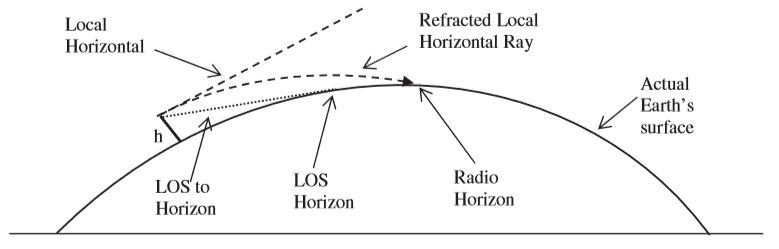
\includegraphics[scale = 0.5]{Figuras/refracao.JPG}
\caption{Efeito da troposfera na direção de propagação da EM, \citep{seybold}}
\end{figure}
\FloatBarrier

\paragraph{}Para facilitar os cálculos na modelagem, convém que se utilize o modelo de Terra Equivalente, pois ele permite que a modelagem seja feita considerando uma trajetória retilínea para os raios. Na modelagem utilizada, a terra possuirá um raio equivalente, tal:

\begin{equation}
    R_T^{eq} = KR_T
    \label{1}
\end{equation}

\paragraph{}Onde $R_T$ é o raio da terra, $R_T^{eq}$ é o raio equivalente da terra e K é o fator de raio equivalente da terra, onde $K = \frac{4}{3}$ para a atmosfera padrão. Assim, temos o seguinte cenário:

\FloatBarrier
\begin{figure}[!htp]
\centering
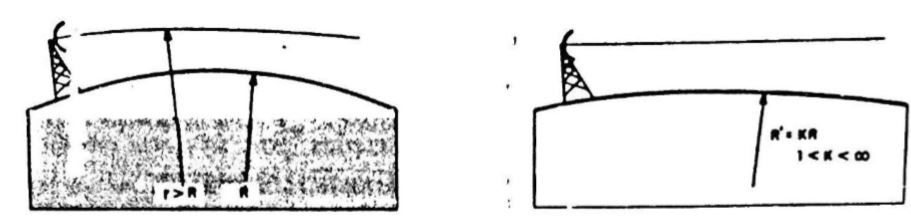
\includegraphics[scale = 0.5]{Figuras/Mod_Terr_Equ.JPG}
\caption{Modelo de Terra Equivalente \citep{Andrezo}}
\end{figure}
\FloatBarrier

\subsection{Distância de Horizonte e Distância do Limiar de Visada}

\paragraph{}Veja a seguinte figura:

\FloatBarrier
\begin{figure}[!htp]
\centering
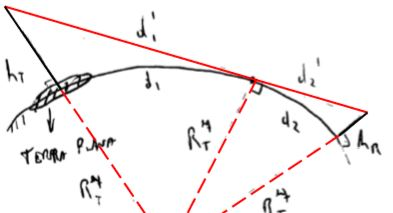
\includegraphics[scale = 0.5]{Figuras/Dist_Hor.JPG}
\caption{Modelo de Terra Equivalente \citep{Andrezo}}
\end{figure}
\FloatBarrier


\paragraph{}Quando $h_T << d_1$ e $h_R << d_2$, então $d1 \approx d'_1$ e $d_2 \approx d'_2$. Assim:

\begin{equation}
    d_1 = d'_1
    \label{2}
\end{equation}

\begin{equation}
    d_1^2 =  (h_T + R_T^{eq})^2 - R_T^{eq2}
    \label{3}
\end{equation}

\begin{equation}    
    d_1 = \sqrt{h_T^2 + 2h_TR_T^{eq}}
    \label{4}
\end{equation}

\paragraph{}Como $h_T << R_T^{eq}$:

\begin{equation}
    d_1 = \sqrt{2h_TR_T^{eq}}
    \label{5}
\end{equation}

\paragraph{}$d_1$ é a distância de horizonte da antena transmissora.

\paragraph{}Analogamente:

\begin{equation}
    d_2 = \sqrt{2h_RR_T^{eq}}
    \label{6}
\end{equation}

\paragraph{}Assim, a distância de visada $d_h$ é definida por:

\begin{equation}
    d_h = d_1 + d_2
    \label{7}
\end{equation}

\begin{equation}
    d_h = \sqrt{2R_T^{eq}}(\sqrt{h_T} + \sqrt{h_R})
    \label{8}
\end{equation}

\paragraph{}Na prática, é aceitável a aproximação de Terra plana ao longo de todo o trecho menor que a distância de horizonte, para cenários sem obstruções. Quando a distância entre as antenas é maior do que a distância de horizonte, se utiliza o modelo de 2 raios para terra esférica \citep{Andrezo}.



\section{Parâmetros fundamentais da Antena}

\subsection{Introdução}Uma antena é definida pelo \textit{IEEE Standard Definitions of Terms for Antennas} como um meio para radiar ou receber ondas rádio. Em outras palavras, a antena é uma estrutura tradicional entre o espaço livre e um dispositivo de guiamento \citep{balanis}. Para descrever o desempenho de uma antena, definições de vários parâmetros são necessários. Dentre eles, os principais que foram utilizados nesse projeto são: a diretividade e o ganho da antena.

\subsection{Diretividade}A diretividade de uma antena $D$ é definida como a razão da intensidade de radiação $U$ numa dada direção da antena com a intensidade de radiação média em todas as direções $U_0$. A intensidade de radiação média é igual a potência total radiada $P_{rad}$ pela antena dividida por 4$\pi$ \citep{balanis}. De forma mais simples, a diretividade  de uma fonte anisotrópica é igual a razão entre sua intensidade de radiação numa dada direção e a intensidade de radiação de uma fonte isotrópica.

\begin{equation}
    D = \frac{U}{U_0}
    \label{9}
\end{equation}

Onde:

\begin{equation}
    U_0 = \frac{P_{rad}}{4\pi}
    \label{10}
\end{equation}

\paragraph{}Portanto:

\begin{equation}
    D = 4\pi\frac{U}{P_{rad}}
    \label{32}
\end{equation}

\paragraph{}A direção de máxima intensidade de radiação (\textit{Diretividade Máxima}) é expressa como:

\begin{equation}
    D_{max} = D_0
    \label{33}
\end{equation}

\begin{equation}
    D_{0} = \frac{4\pi U_{max}}{P_{rad}}
    \label{34}
\end{equation}

\subsection{Ganho}

\paragraph{}Outra medida eficiente que descreve o desempenho da antena é o seu \textit{ganho}. Embora o ganho da antena esteja diretamente relacionado à diretividade, é uma medida que leva em consideração tanto a eficiência da antena como suas capacidades direcionais.

\paragraph{}O ganho de uma antena numa dada direção $G(\theta, \phi)$ é definido pela razão da intensidade numa dada direção $U(\theta, \phi)$, com a intensidade de radiação que seria obtida se a potência aceita pela antena fosse radiada isotropicamente \citep{balanis}. A intensidade de radiação correspondente a potência radiada isotropicamente é igual a potência de entrada da antena $P_{in}$, dividida por $4\pi$.

\begin{equation}
    G(\theta, \phi) = 4\pi\frac{U(\theta,\phi)}{P_{in}}
    \label{35}
\end{equation}

\paragraph{}A potência radiada relaciona-se com a potência de entrada na antena através da seguinte relação:

\begin{equation}
    P_{rad} = e_{cd}P_{in}
    \label{36}
\end{equation}

\paragraph{}Onde $e_{cd}$ é a eficiência de radiação (adimensional).

\paragraph{}Substituindo $P_{in}$ da equação \ref{36}, na equação \ref{35}, temos que:

\begin{equation}
    G(\theta, \phi) = e_{cd}[4\pi\frac{U(\theta, \phi)}{P_{rad}}]
    \label{37}
\end{equation}

\paragraph{}Que está relacionado a diretividade por:

\begin{equation}
    G(\theta,\phi) = e_{cd}D(\theta,\phi)
    \label{39}
\end{equation}

\subsection{Dipolo de meia onda}

\paragraph{}A antena dipolo de meia onda é uma das mais utilizadas atualmente em várias aplicações, principalmente porque a sua resistência de radiação é 73 ohms, que é bem próxima dos 50-ohm ou 75-ohm das impedâncias características de algumas linhas de transmissão \citep{balanis}.

\paragraph{} A intensidade de radiação de um dipolo de meia onda, alimentada por uma corrente $I_0$ e impedância característica $\eta$, é dada por \citep{balanis}:


\begin{equation}
    U(\theta) = \eta \frac{|I_0|^2}{8\pi^2}\sin^3\theta
    \label{40}
\end{equation}

\paragraph{}E a sua potência de radiação é dada por:

\begin{equation}
    P_{rad} = \eta \frac{|I_0|^2}{8\pi}C_{in}(2/pi)
    \label{41}
\end{equation}

\paragraph{}
Onde $C_{2\pi} = 2.435$ \citep{balanis}.


\paragraph{}Substituindo as expressões \ref{41} e \ref{40}, em \ref{34}, temos que:

\begin{equation}
    D(\theta,\phi) \approx 1.643\sin^3 \theta
    \label{42}
\end{equation}

\begin{equation}
    D(\theta) \approx 1.643\sin^3 \theta
    \label{43}
\end{equation}



\paragraph{}Portanto, substituindo a expressão \ref{43} na expressão \ref{39}, temos :

\begin{equation}
\label{Ganho}
    G(\theta,\phi) = 1.643e_{cd}\sin^3\theta
\end{equation}

\section{Modelo de dois raios}

\FloatBarrier
\begin{figure}[!htp]
\centering
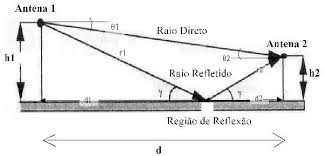
\includegraphics[scale = 0.8]{Figuras/images.jpg}
\caption{Modelo de 2 Raios Terra Plana}
\end{figure}
\FloatBarrier



\paragraph{}Nesse modelo, existem duas antenas, sendo uma transmissora de altura $h_t = h_1$ e uma receptora de altura $h_r = h_2$, separadas por uma distância d. O meio possui uma condutividade $\sigma$ e desvio-padrão das irregularidades de altura $\Delta h$. Nesse modelo, dado que a polarização da onda é perpendicular, o campo elétrico no receptor é expresso por:

\begin{equation}
\label{Mod2Raios}
    E = e^{-j\beta r_d}(E_{0d}F_{T}(\theta_i^{Tx})F_{R}(\theta_i^{Rx})+E_{0r}F_{T}(\theta_r^{Tx})F_{R}(\theta_r^{Rx})\rho_s\Gamma(\theta)e^{-j\beta\triangle r_d})
\end{equation}

\paragraph{}Sendo E o campo elétrico resultante da interferência entre o campo elétrico refletido no solo, e o campo elétrico que se propaga diretamente da antena transmissora. $E_{0d}$ e $E_{0r}$ são os campos elétricos que se propagam no ar livre, direto e refletido, respectivamente, dados por:

\begin{equation}
    {E_{Od}}^2 = \frac{30EIRP}{r_d^2}
\end{equation}

\begin{equation}
    {E_{Or}}^2 = \frac{30EIRP}{r_r^2}
\end{equation}

\paragraph{}Onde EIRP (\textit{Effective Isotropic Radiated Power}) é a potência efetivamente radiada. Ela é função da potência transmitida $P_t$:

\begin{equation}
    EIRP = P_tG_t
\end{equation}


\paragraph{}Na expressão \ref{Mod2Raios}, $F_x(\theta)$ é a função de radiação direcional da antena x, $\theta_i^{Tx}$ e $\theta_r^{Tx}$ são os ângulos de azimute com a direção da antena em relação a vertical e $\Delta r$ é a diferença de percurso entre o raio direto $r_d$ e o refletido $r_r$. 



\paragraph{} O coeficiente de reflexão $\Gamma(\theta)$ depende do meio no qual ocorre a propagação, e do ângulo de incidência da onda refletida $\theta_i$. A sua expressão depende também do tipo de polarização da onda:



\paragraph{}Para polarização perpendicular:

\begin{equation}
    \Gamma(\theta_i) = \frac{cos\theta_i - \sqrt{\frac{\epsilon_{1c}}{\epsilon_{2c}}}\sqrt{1 - \frac{\epsilon_{2c}}{\epsilon_{1c}}{sen\theta_i}^2}}{cos\theta_i + \sqrt{\frac{\epsilon_{1c}}{\epsilon_{2c}}}\sqrt{1 - \frac{\epsilon_{2c}}{\epsilon_{1c}}{sen\theta_i}^2}}
\end{equation}



\paragraph{}Para polarização horizontal:

\begin{equation}
    \Gamma(\theta_i) = \frac{-\cos\theta_i + \sqrt{\frac{\epsilon_{1c}}{\epsilon_{2c}}}\sqrt{1 - \frac{\epsilon_{1c}}{\epsilon_{2c}}{\sin\theta_i}^2}}{\cos\theta_i + \sqrt{\frac{\epsilon_{1c}}{\epsilon_{2c}}}\sqrt{1 - \frac{\epsilon_{1c}}{\epsilon_{2c}}{\sin\theta_i}^2}}
\end{equation}


\paragraph{}A relação do coeficiente de reflexão com o meio está expresso na permissividade complexa, que é dada por:

\begin{equation}
    \epsilon_c = \epsilon - j\frac{\sigma}{\omega}
\end{equation}

\paragraph{}Onde $\epsilon$ é a permissividade do meio, e $\omega = 2\pi f$, sendo f a frequência na qual a onda está se propagando.

\paragraph{}Por fim, deve-se levar em consideração a perda devido á rugosidade do solo. Para isso, é feita a análise do critério de Raylegh. Onde analisamos a diferença de fase entre as frentes de onda refletidas pela superfície $\triangle\phi$, sendo \citep{Andrezo}:

\begin{equation}
    \triangle\phi = \frac{4\pi\Delta hcos\theta_i}{\lambda}
\end{equation}

\paragraph{}Se $\triangle\phi < \frac{\pi}{2}$, conclui-se que a superfície é lisa, não havendo necessidade de levar em consideração a perda por rugosidade.

\paragraph{}Se $\triangle\phi > \frac{\pi}{2}$, a perda por rugosidade deverá ser levada em consideração, multiplicando-se o coeficiente de reflexão pelo fator de perda por espalhamento $\rho_s$:

\begin{equation}
    \rho_s = e^{-0.5{\Delta \phi}^2}
\end{equation}

\paragraph{}Dessa forma, ao se analisar a propagação das ondas eletromagnéticas num determinado meio, serão aferidos quais os efeitos, tanto do meio, caracterizados pela perda por propagação no espaço livre, reflexão no solo e pela rugosidade do mesmo, quanto das características da própria antena, tais como altura e polarização.

\paragraph{}No presente trabalho, será analisada para alguns cenários, a potência recebida pela antena receptora $P_r$. Calcularemos ela, utilizando a densidade de potência irradiada $S$ por uma antena no espaço livre:

\begin{equation}
    S = \frac{|E|^2}{120\pi}
\end{equation}

E a área efetiva da antena receptora $A_{em}$ \cite{balanis}:

\begin{equation}
    A_{ef} = \frac{\lambda^2G_r}{4\pi}
\end{equation}

\paragraph{}Finalmente:

\begin{equation}
    P_r = SA_{ef}
\end{equation}
